\chapter{Implementing flow-level model}
\label{chapter:implementation}

In this chapter we start by describing how we started the implementation task, we then move to the discussion of the implementation details. Finally, we present the final version of the implemented flow-level model. 

By definition, as we have shown in Equation~\ref{eq:2.1}, the energy consumption of a given electronic equipment is given by the product of the average power drawn by the equipment and its time duration of running. We have also shown, in Figure~\ref{fig:energyproportionality} and Equation~\ref{eq:2.2}, the linear relationship that exist between network equipment load and power consumption. Combining Equation~\ref{eq:2.1} and Equation~\ref{eq:2.2}, we get Equation~\ref{eq:5.1} for energy consumption of a given device for a given time duration of T, where \($$P_{idle}$$\) is the power that the equipment consumed when there is no traffic and \(P_{dynamic}\) is the additional power drawn due to network traffic.

\begin{equation} \label{eq:5.1}
E(T) =  \int_{0}^{T} (P_{idle} + P_{dynamic})(t) dt 
\end{equation} 

To implement this model in SimGrid, we need to determine the values of the three variables shown in Equation~\ref{eq:5.1}. We can directly read the idle power consumption value from the SimGrid's link property that we described in Section~\ref{section:simgridenvironment}. For the \(P_{dynamic}\), we need to describe how SimGrid compute load in its core. 

Briefly described, for a set of simulated activities running on a given simulated network resource such as a switch, SimGrid computes, using its bandwidth sharing algorithm, the amount of resource share that each activity can get. The sum of the resource share that all activities can get for a given resource at a given moment cannot exceed the capacity of the resource on which the activities are running. Figure~\ref{fig:SimGrid} depicts this concept symbolically. We can access how much of the resource is currently in use, i.e., its load, from SimGrid's core library. SimGrid dynamically recompute the resource usage when any of the allocated activities finish their data transfer task. 

We can compute the dynamic power consumption, \(P_{dynamic}\), of a link at any given instance as shown in equation Equation~\ref{eq:5.2}. Similar to the idle value, we can read the busy power consumption value,\(P_{busy}\), directly from the 
Link property description and u is link utilization computed by dividing the load (used bandwidth) by the maximum bandwidth. The maximum bandwidth value is also available on the Link description. 

\begin{equation} \label{eq:5.2}
P_{dynamic} = (P_{busy} - P_{idle}) * u 
\end{equation} 
where:
\begin{description}
    \item [u]: is a normalized utilization factor obtained by dividing the current Link load with its full capacity, and 
    \item [(\($$P_{busy} - P_{idle}$$\))]: is the slope of the relationship between load and power consumption as shown in Figure~\ref{fig:energyproportionality}.
\end{description} 
In Chapter~\ref{chapter:environment}, we mentioned that SimGrid provides an interface to NS-3. In order to take advantage of this feature, especially during the validation phase, we took into account how the SimGrid's links are mapped to NS-3's abstraction. We found out that for each Link abstraction of SimGrid, two NetDevices are created in NS-3. Therefore, the idle and busy values of the Link shown in Equation~\ref{eq:5.2} are multiplied by two.

To compute the total energy, \(E(T)\), of a network during the time interval T, the approach we followed is that each time when an event happens on a link (link created or destroyed, link turned on or off, or link load change, or simulation ended), we read the link load and multiply it by the time elapsed between the current event and the previous event. This gives us the energy consumed between two events. We collect this value for all events happened during time duration T for each link and finally, when the simulation ends, we collect all the energy values for all the links. This value gives us the total energy consumption, \(E(T)\) of the simulated network.

One major problem that we faced during our preliminary validation experiment of this implementation is that there is discrepancy between the simulated time value of SimGrid and ECOFEN. Figure~\ref{fig:bandwidthvstime} shows this discrepancy when 200 mega bytes of data is transfered at different bandwidth level (ranging between 10 and 500 Mbps). Approximately, as shown in the figure, for bandwidth value of below 100 Mbps both simulators seems to agree on the simulated time but above 100 Mbps, ECOFEN stays constant while SimGrid keeps on decreasing at a slower rate. We have also confirmed that the time predictions stays close below 100 Mbps for varying data sizes (20 to 500 Mbytes) by testing at two different bandwidth values (10 and 50 Mbps).

\begin{figure}[ht]
	\begin{center}
		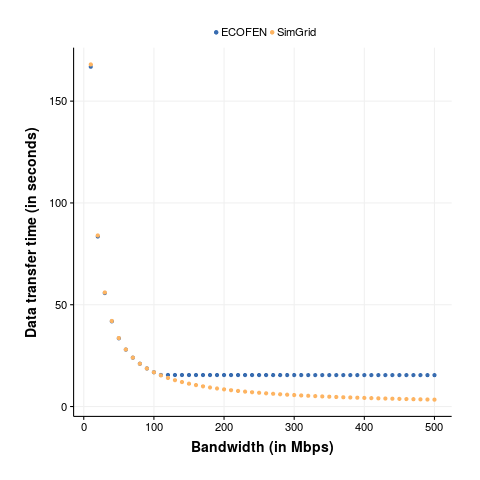
\includegraphics[width=14cm]{images/ex18_bw_time_sg_vs_ns3}
		\caption{Simulated time required to transferr 100 Mbytes of data at different bandwidth settings: comparison between ECOFEN and SimGrid simulators}
		\label{fig:bandwidthvstime}
	\end{center}
\end{figure}

Since the model shown in Equation~\ref{eq:5.1} depends on time value and since we are also going to validate this model against ECOFEN, for all accuracy and scalability validation experiments presented in the next chapter, we decided to use bandwidth values residing below 100 Mbps where both SimGrid and ECOFEN seems to agree. The task of figuring out why these two simulators seems to predict time differently is beyond the scope of this work. 

